Para este caso, o stent farmacológico é colocado na parte superior 
do canal curvado. O mesmo é modelado por 10 semi círculos uniformemente
espaçados. Assim como no caso anterior, foi considerado uma obstrução
de 40\% do canal devido a aterosclerose e o domínio foi
discretizado com 15875 nós e 35408 elementos triangulares lineares. \par
A \ref{velocity evolution curved stent} apresenta o perfil
de velocidade transiente ao longo da coordenada $y$ no
meio do canal ($x=5R$). 
Como podemos observar, 
o valor adimensional máximo do campo de velocidade
chega a $u=3.6$ quando o stent é implantado, isto é,
possuímos um aumento de $56$\% quando comparado com
a artéria apenas com aterosclerose como no caso anterior (ver seção \ref{canal curvado}).

\begin{figure}[H]
     \centering
     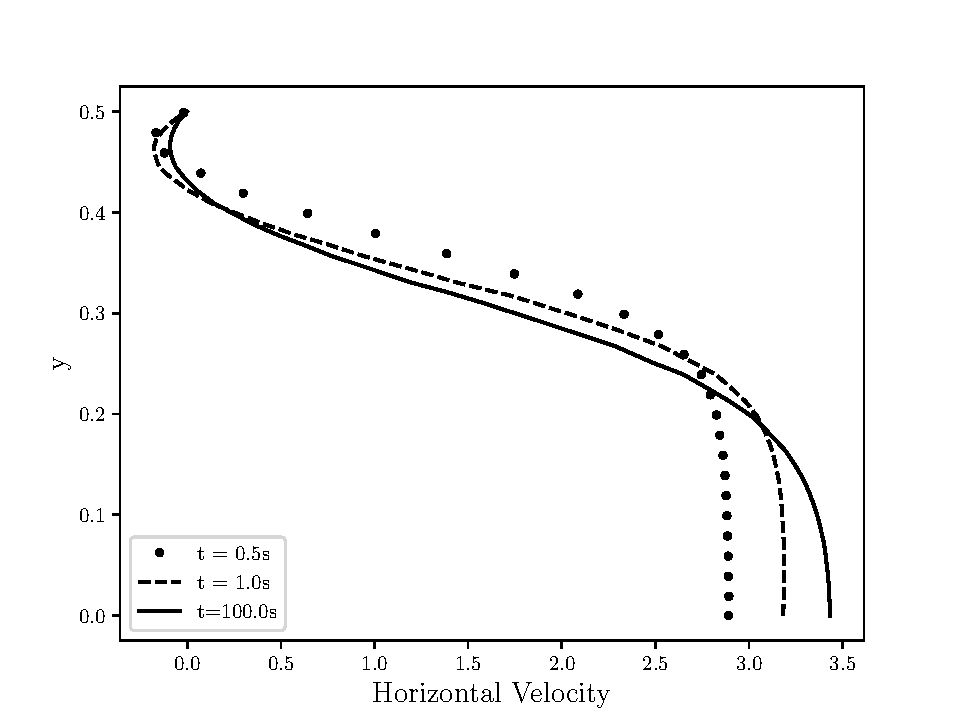
\includegraphics[scale=1]{./02_chaps/cap_solution/figure/vel_CurvedStrut_evol.pdf}\\
     \caption{Evolução no tempo do perfil da velocidade para o Canal Curvado com Stent Farmacológico.}
     \label{velocity evolution curved stent}
\end{figure}

\newpage
A \ref{velocity field curved stent} apresenta a evolução no tempo e no espaço
do campo de velocidade para a metade do domínio já que os resultados são simétricos
na direção $y$. O campo de velocidade é representado com os valores adimensionais
onde a cor vermelha se refere ao valor $u=3.6$ e a cor azul $u=0$. 
Transformando em valores dimensionais temos $u=43.2 cm/s$ e $u=0 cm/s$ respectivamente. 

\vspace{2cm} 
\begin{figure}[H]
     \begin{minipage}{.50\linewidth}
      \centering
      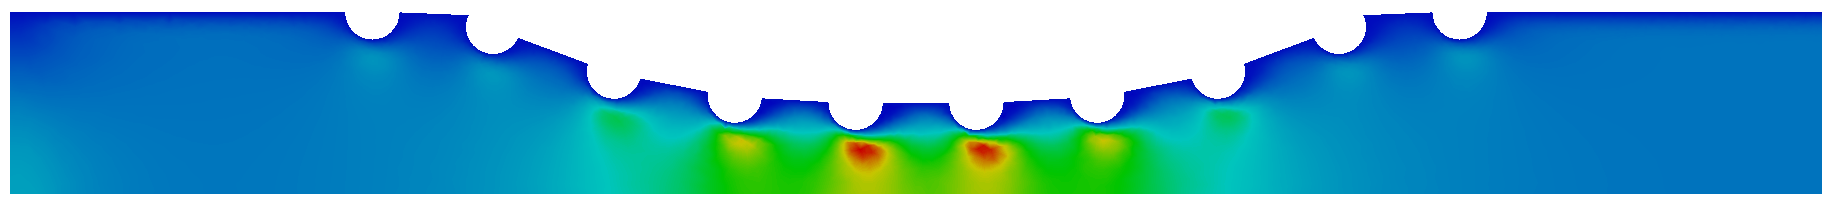
\includegraphics[scale=0.12]{./02_chaps/cap_solution/figure/vel_CurvedStrut200.png}\\
      t = 0.1
     \end{minipage}%
     \begin{minipage}{.50\linewidth}
      \centering
      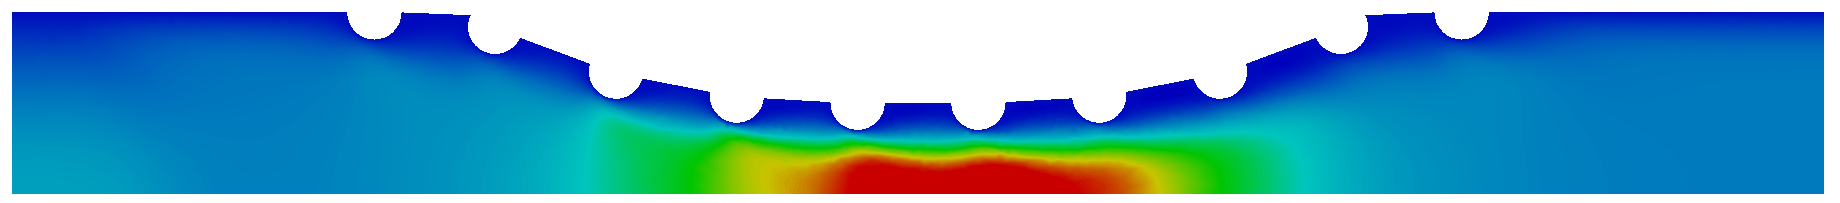
\includegraphics[scale=0.12]{./02_chaps/cap_solution/figure/vel_CurvedStrut1000.png}\\
      t = 0.5
     \end{minipage}
     \begin{minipage}{.50\linewidth}
     \medskip
      \centering
      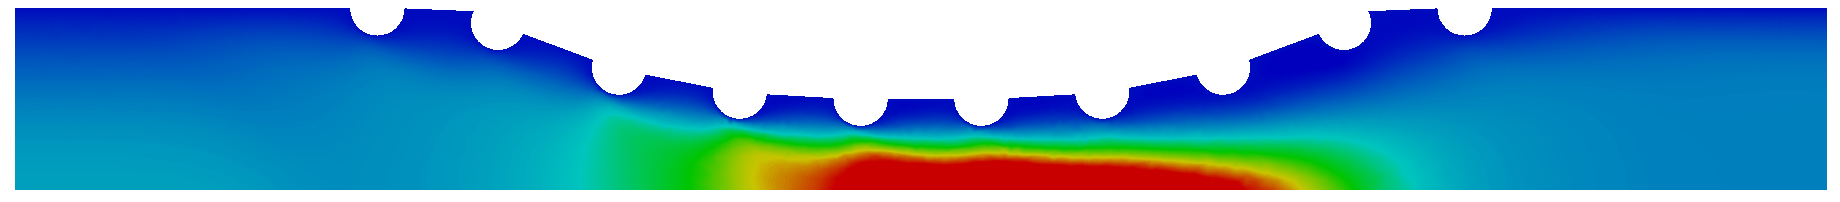
\includegraphics[scale=0.12]{./02_chaps/cap_solution/figure/vel_CurvedStrut2000.png}\\
      t = 1.0
     \end{minipage}%
     \begin{minipage}{.50\linewidth}
     \medskip
      \centering
      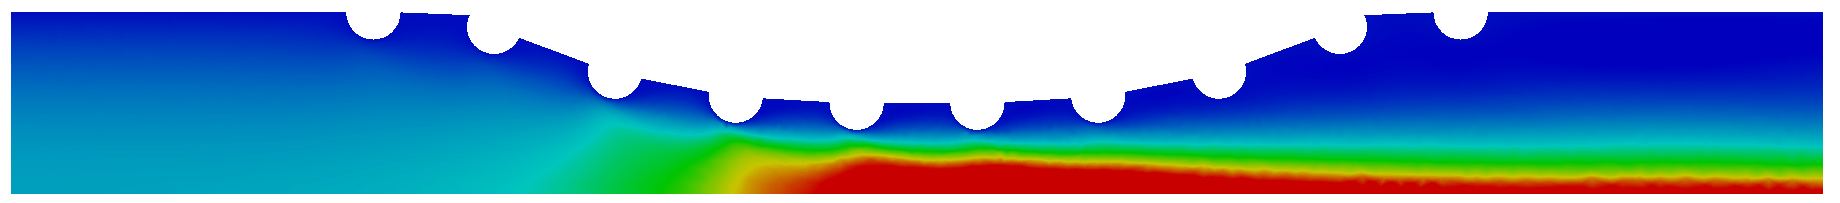
\includegraphics[scale=0.12]{./02_chaps/cap_solution/figure/vel_CurvedStrut6000.png}\\
      t = 3.0
     \end{minipage}
     \begin{minipage}{.50\linewidth}
      \centering
      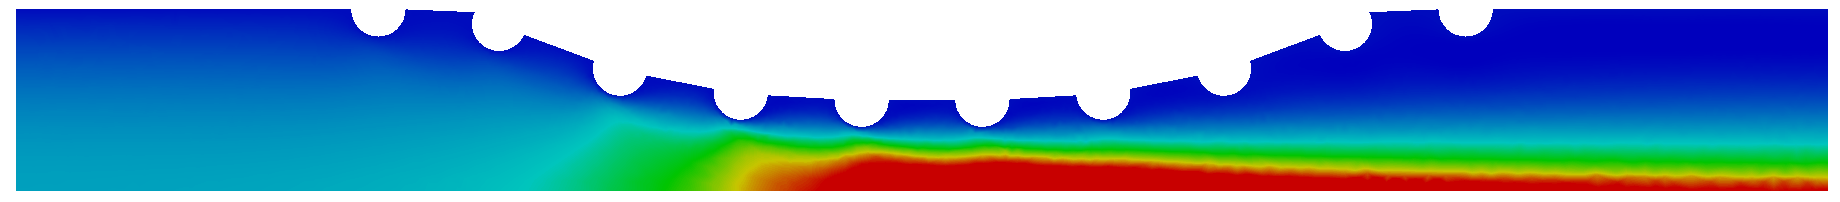
\includegraphics[scale=0.12]{./02_chaps/cap_solution/figure/vel_CurvedStrut8000.png}\\
      t = 4.0
     \end{minipage}%
     \begin{minipage}{.50\linewidth}
      \centering
      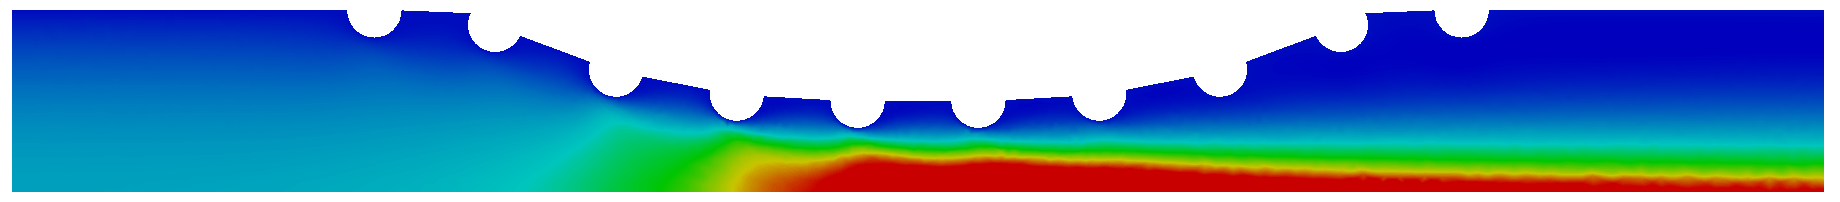
\includegraphics[scale=0.12]{./02_chaps/cap_solution/figure/vel_CurvedStrut10000.png}\\
      t = 5.0
     \end{minipage}
     \begin{minipage}{.50\linewidth}
     \medskip
      \centering
      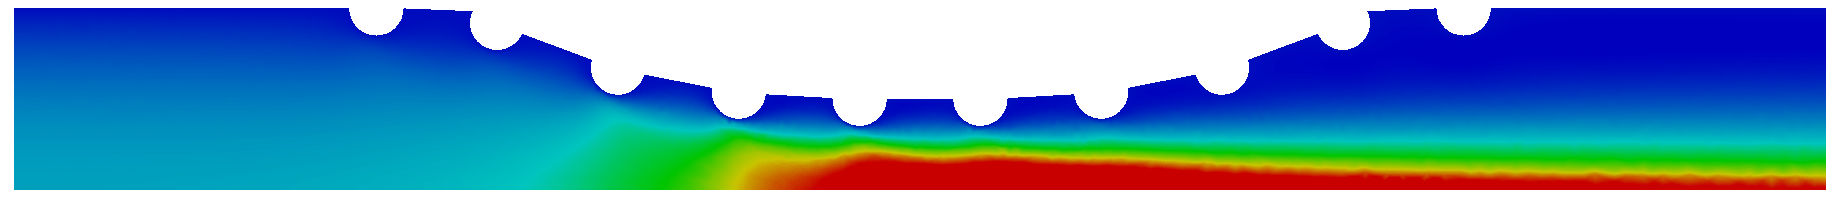
\includegraphics[scale=0.12]{./02_chaps/cap_solution/figure/vel_CurvedStrut14000.png}\\
      t = 7.0
     \end{minipage}%
     \begin{minipage}{.50\linewidth}
     \medskip
      \centering
      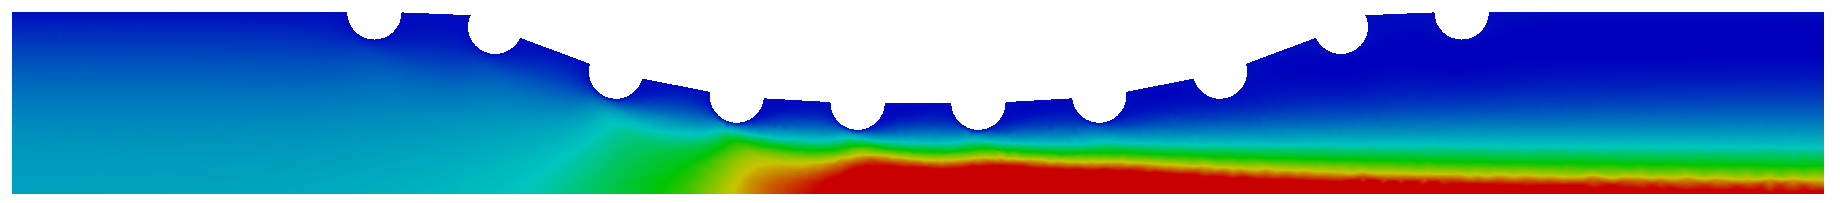
\includegraphics[scale=0.12]{./02_chaps/cap_solution/figure/vel_CurvedStrut20000.png}\\
      t = 10.0
     \end{minipage}
     \medskip
     \caption{Evolução no tempo e no espaço do campo de velocidade para o Canal Curvado com Stent Farmacológico.}
     \label{velocity field curved stent}
\end{figure}


\vspace{1cm}
Conforme mencionado por Lucena et al. (2017) \cite{lucena2017}, é estimado que $47$\% do fármaco é difundido na corrente sanguínea.
A \ref{conc field curved stent sc 1} e a \ref{conc field curved stent sc 10} 
apresentam a evolução no tempo e no espaço
do campo da concentração para a metade do domínio devido a simetria para diversos números de \textit{Schmidt}
tais como: $1$ e $10$ respectivamente.
A concentração é representado com os valores adimensionais
onde a cor vermelha representa $100$\% e a cor azul representa $0$\% 
dessa concentração que é difundida na corrente sanguínea. 
É possível observar que o número de Schmidt influencia
diretamente no transporte do fármaco na corrente sanguínea. Para elevados valores do
número de \textit{Schmidt}, o transporte de espécie química torna-se puramente convectivo.

\begin{figure}[H]
     \begin{minipage}{.50\linewidth}
      \centering
      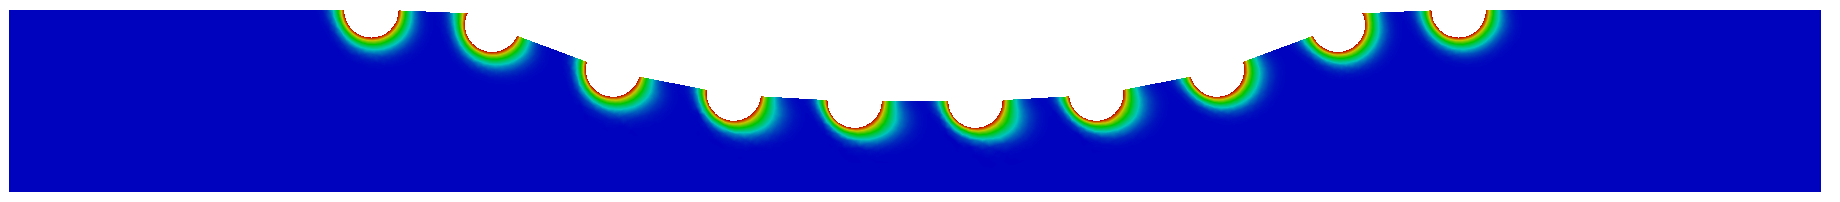
\includegraphics[scale=0.12]{./02_chaps/cap_solution/figure/conc1_CurvedStrut200.png}\\
      t = 0.1
     \end{minipage}%
     \begin{minipage}{.50\linewidth}
      \centering
      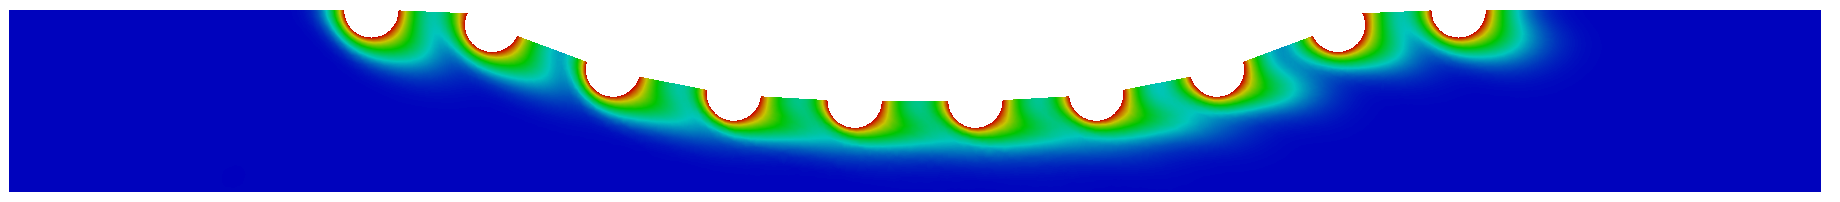
\includegraphics[scale=0.12]{./02_chaps/cap_solution/figure/conc1_CurvedStrut1000.png}\\
      t = 0.5
     \end{minipage}
     \begin{minipage}{.50\linewidth}
     \medskip
      \centering
      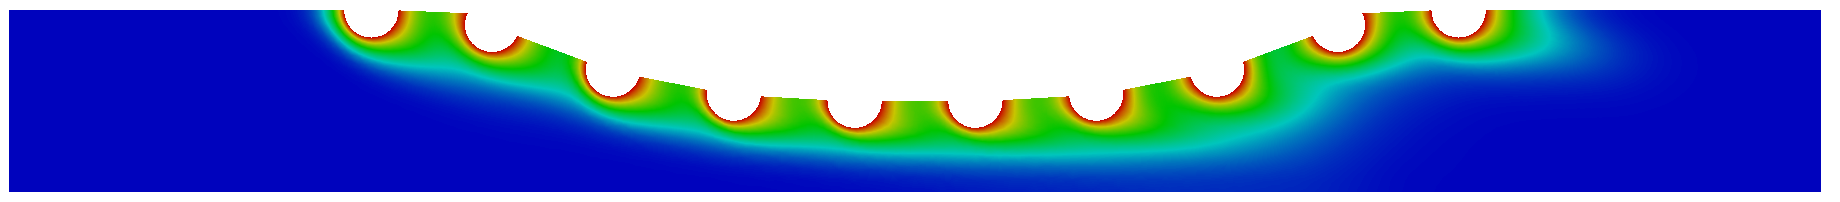
\includegraphics[scale=0.12]{./02_chaps/cap_solution/figure/conc1_CurvedStrut2000.png}\\
      t = 1.0
     \end{minipage}%
     \begin{minipage}{.50\linewidth}
     \medskip
      \centering
      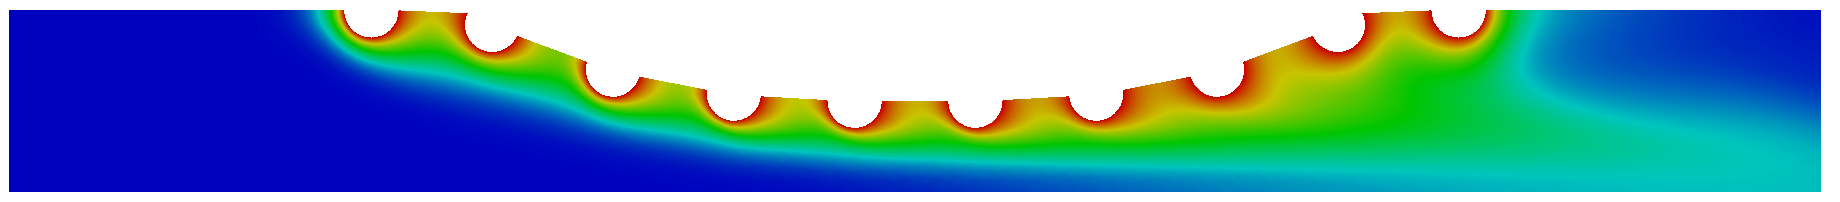
\includegraphics[scale=0.12]{./02_chaps/cap_solution/figure/conc1_CurvedStrut6000.png}\\
      t = 3.0
     \end{minipage}
     \begin{minipage}{.50\linewidth}
      \centering
      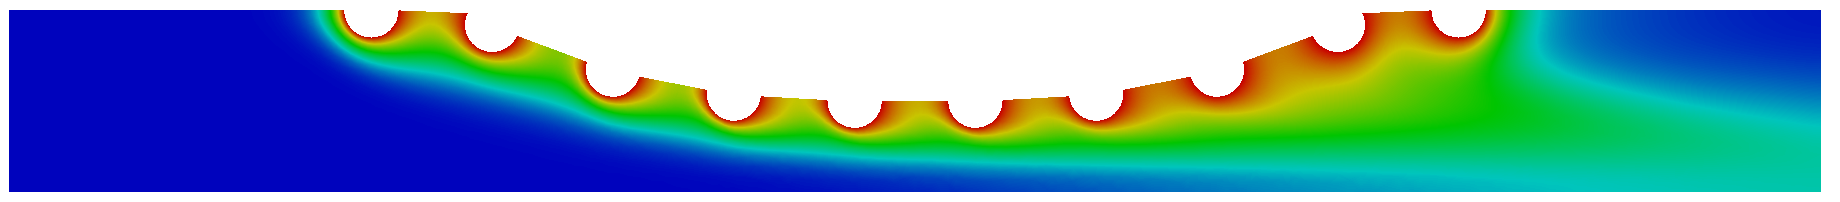
\includegraphics[scale=0.12]{./02_chaps/cap_solution/figure/conc1_CurvedStrut8000.png}\\
      t = 4.0
     \end{minipage}%
     \begin{minipage}{.50\linewidth}
      \centering
      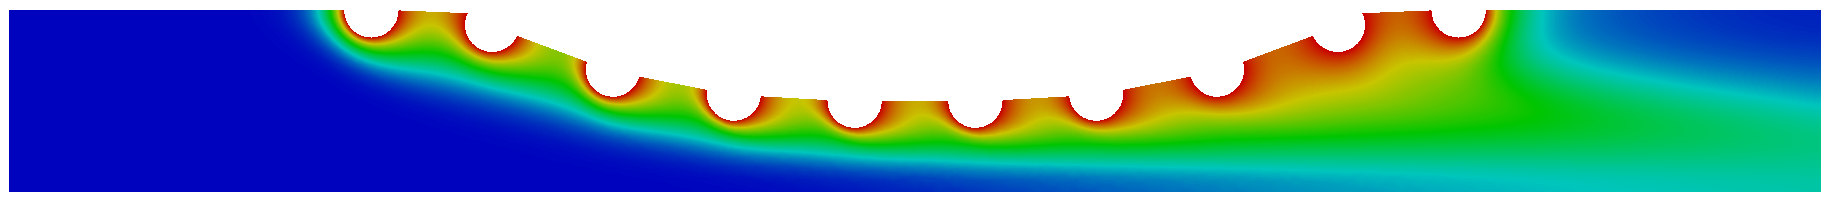
\includegraphics[scale=0.12]{./02_chaps/cap_solution/figure/conc1_CurvedStrut10000.png}\\
      t = 5.0
     \end{minipage}
     \begin{minipage}{.50\linewidth}
     \medskip
      \centering
      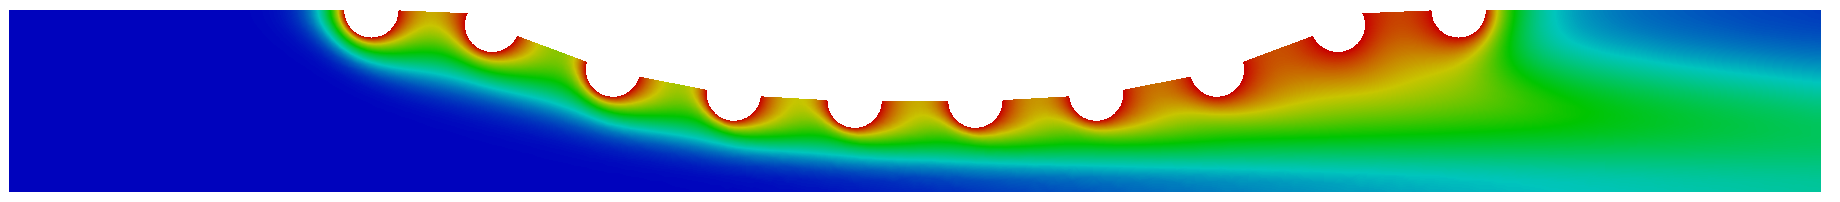
\includegraphics[scale=0.12]{./02_chaps/cap_solution/figure/conc1_CurvedStrut14000.png}\\
      t = 7.0
     \end{minipage}%
     \begin{minipage}{.50\linewidth}
     \medskip
      \centering
      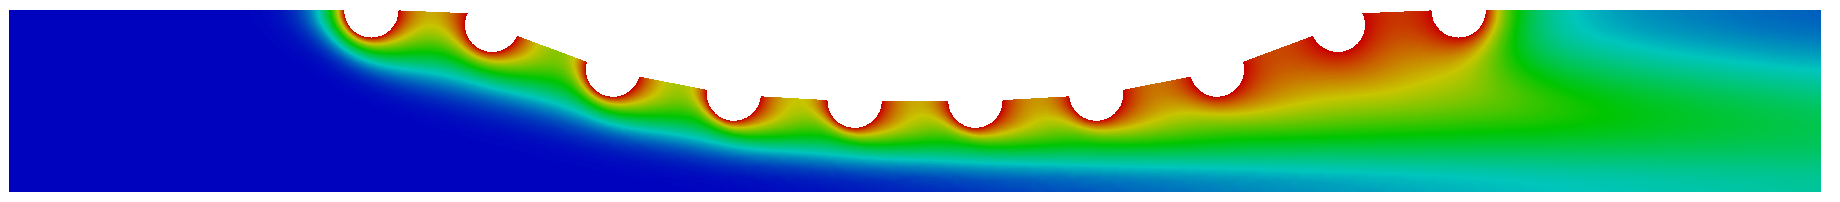
\includegraphics[scale=0.12]{./02_chaps/cap_solution/figure/conc1_CurvedStrut20000.png}\\
      t = 10.0
     \end{minipage}
     \medskip
     \caption{Evolução no tempo e no espaço do campo de espécie química para o Canal Curvado com Stent Farmacológico com $Sc=1$.}
     \label{conc field curved stent sc 1}
\end{figure}

\bigskip
\begin{figure}[H]
     \begin{minipage}{.50\linewidth}
      \centering
      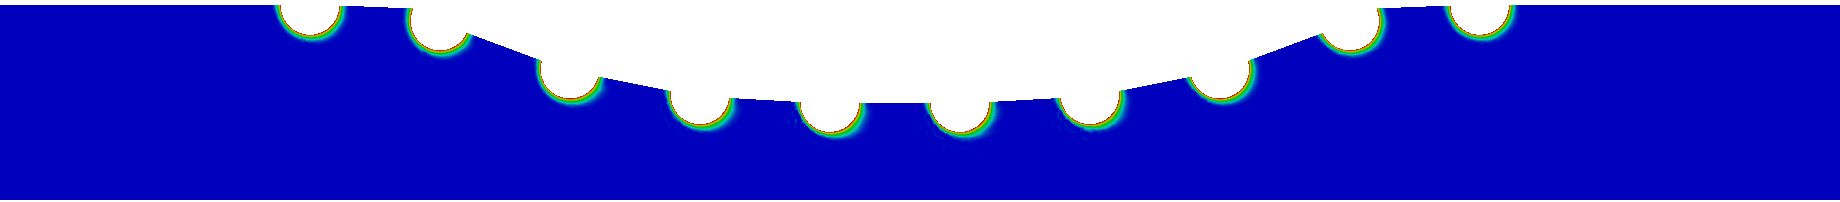
\includegraphics[scale=0.12]{./02_chaps/cap_solution/figure/conc10_CurvedStrut500.png}\\
      t = 0.1
     \end{minipage}%
     \begin{minipage}{.50\linewidth}
      \centering
      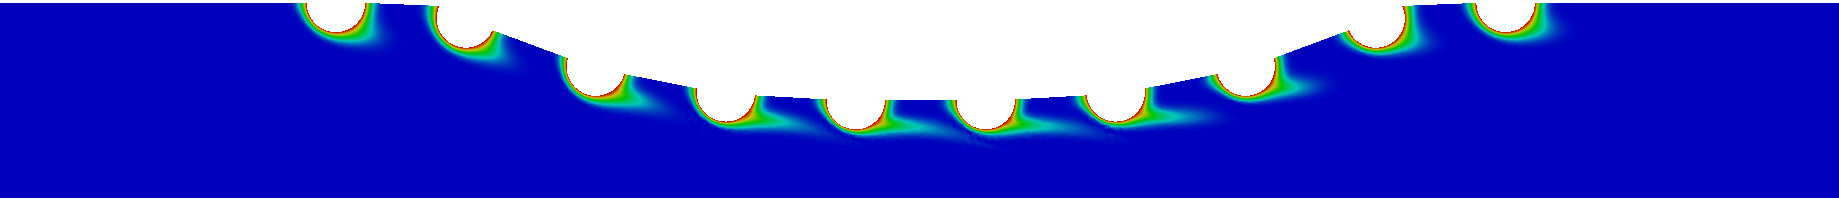
\includegraphics[scale=0.12]{./02_chaps/cap_solution/figure/conc10_CurvedStrut2500.png}\\
      t = 0.5
     \end{minipage}
     \begin{minipage}{.50\linewidth}
     \medskip
      \centering
      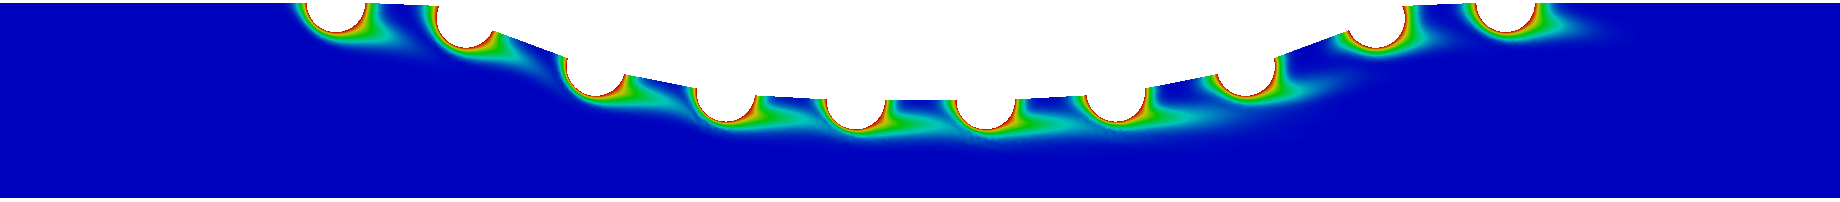
\includegraphics[scale=0.12]{./02_chaps/cap_solution/figure/conc10_CurvedStrut5000.png}\\
      t = 1.0
     \end{minipage}%
     \begin{minipage}{.50\linewidth}
     \medskip
      \centering
      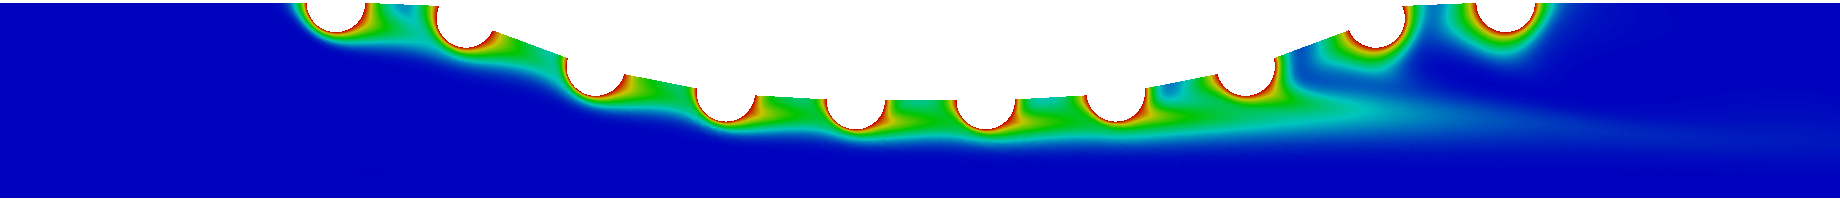
\includegraphics[scale=0.12]{./02_chaps/cap_solution/figure/conc10_CurvedStrut15000.png}\\
      t = 3.0
     \end{minipage}
     \begin{minipage}{.50\linewidth}
      \centering
      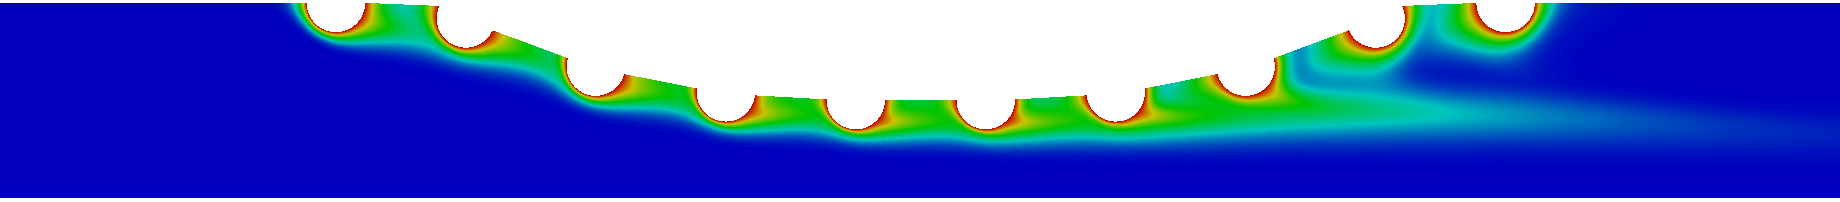
\includegraphics[scale=0.12]{./02_chaps/cap_solution/figure/conc10_CurvedStrut20000.png}\\
      t = 4.0
     \end{minipage}%
     \begin{minipage}{.50\linewidth}
      \centering
      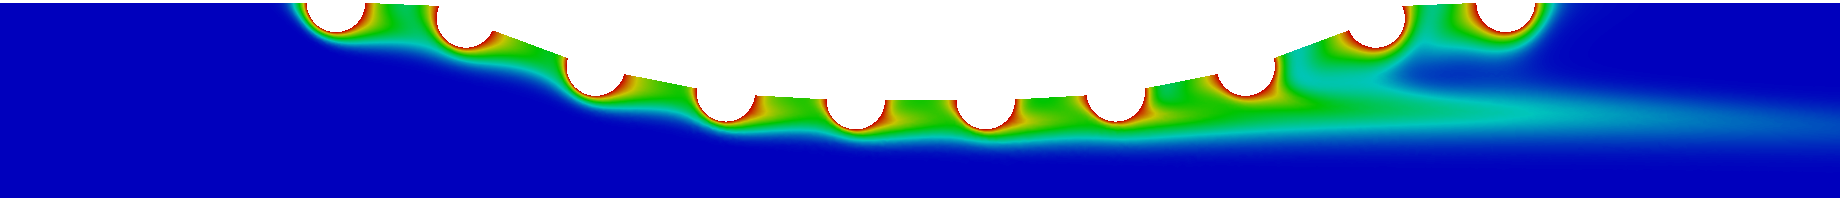
\includegraphics[scale=0.12]{./02_chaps/cap_solution/figure/conc10_CurvedStrut25000.png}\\
      t = 5.0
     \end{minipage}
     \begin{minipage}{.50\linewidth}
     \medskip
      \centering
      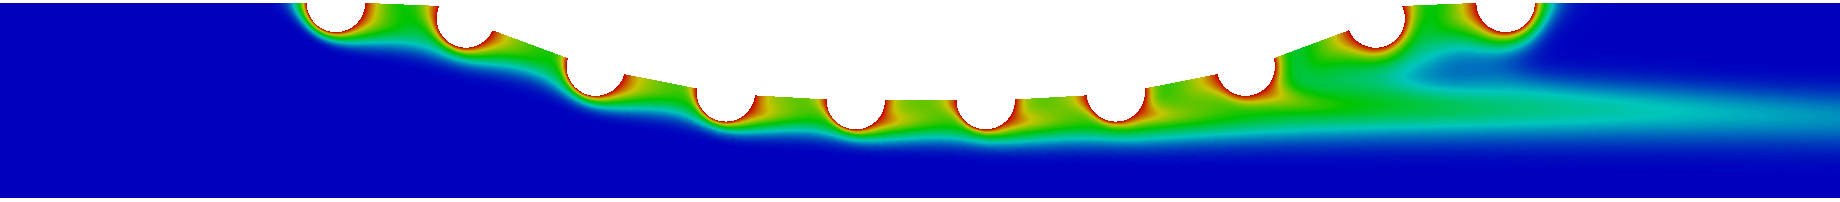
\includegraphics[scale=0.12]{./02_chaps/cap_solution/figure/conc10_CurvedStrut35000.png}\\
      t = 7.0
     \end{minipage}%
     \begin{minipage}{.50\linewidth}
     \medskip
      \centering
      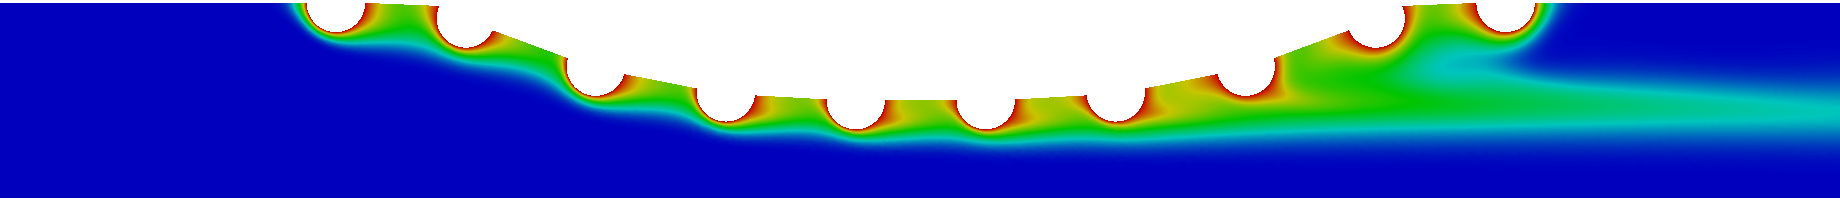
\includegraphics[scale=0.12]{./02_chaps/cap_solution/figure/conc10_CurvedStrut50000.png}\\
      t = 10.0
     \end{minipage}
     \medskip
     \caption{Evolução no tempo e no espaço do campo de espécie química para o Canal Curvado com Stent Farmacológico com $Sc=10$.}
     \label{conc field curved stent sc 10}
\end{figure}

\medskip
